\documentclass[twoside,twocolumn]{article}

\usepackage{blindtext} % Package to generate dummy text throughout this template 
\usepackage{graphicx}
\usepackage[sc]{mathpazo} % Use the Palatino font
\usepackage[T1]{fontenc} % Use 8-bit encoding that has 256 glyphs
\linespread{1.05} % Line spacing - Palatino needs more space between lines
\usepackage{microtype} % Slightly tweak font spacing for aesthetics

\usepackage[english]{babel} % Language hyphenation and typographical rules

\usepackage[hmarginratio=1:1,top=32mm,columnsep=20pt]{geometry} % Document margins
\usepackage[hang, small,labelfont=bf,up,textfont=it,up]{caption} % Custom captions under/above floats in tables or figures
\usepackage{booktabs} % Horizontal rules in tables
\usepackage{graphicx}
\usepackage{lettrine} % The lettrine is the first enlarged letter at the beginning of the text

\usepackage{enumitem} % Customized lists
\setlist[itemize]{noitemsep} % Make itemize lists more compact

\usepackage{abstract} % Allows abstract customization
\renewcommand{\abstractnamefont}{\normalfont\bfseries} % Set the "Abstract" text to bold
\renewcommand{\abstracttextfont}{\normalfont\small\itshape} % Set the abstract itself to small italic text

\usepackage{titlesec} % Allows customization of titles

\titleformat{\section}[block]{\large\scshape\centering}{\thesection.}{1em}{} % Change the look of the section titles
\titleformat{\subsection}[block]{\large}{\thesubsection.}{1em}{} % Change the look of the section titles

\usepackage{fancyhdr} % Headers and footers
\pagestyle{fancy} % All pages have headers and footers
\fancyhead{} % Blank out the default header
\fancyfoot{} % Blank out the default footer
\fancyhead[C]{Comparativa de las metodologìas de elaboración de Datawarehouse vs metodologias de elaboración de Datalakes $\bullet$ Abril 2022 $\bullet$ } % Custom header text
\fancyfoot[RO,LE]{\thepage} % Custom footer text

\usepackage{titling} % Customizing the title section

\usepackage{hyperref} % For hyperlinks in the PDF

%----------------------------------------------------------------------------------------
%	TITLE SECTION
%----------------------------------------------------------------------------------------
\providecommand{\keywords}[1]{
  \small	
  \textbf{\textit{\quad \quad Keywords: }} #1}

\providecommand{\pclave}[1]{
  \small	
  \textbf{\textit{\quad \quad Palabras Clave: }} #1}

%Idiomas: \selectlanguage{english} \selectlanguage{spanish}

\begin{document}

\title{Trabajo Encargado 04:Comparativa de las metodologìas de elaboración de Datawarehouse vs metodologias de elaboración de Datalakes}

\begin{titlepage}
\begin{figure}[htb]
\begin{center}

\includegraphics[width=5cm]{imagenes/logo.png}
\end{center}    
\end{figure}
\vspace*{-0.25in}
\begin{center}
\large{UNIVERSIDAD PRIVADA DE TACNA}\\
\vspace*{-0.025in}
INGENIERIA DE SISTEMAS  \\	

\vspace*{0.5in}
\begin{large}
TITULO:\\
\end{large}

\vspace*{0.1in}
\begin{Large}
\textbf{ Comparativa de las metodologìas de elaboración de Datawarehouse vs metodologias de elaboración de Datalakes} \\
\end{Large}

\vspace*{0.3in}
\begin{Large}
\textbf{CURSO:} \\
\end{Large}

\vspace*{0.1in}
\begin{large}
Inteligencia de Negocios\\
\end{large}

\vspace*{0.3in}
\begin{Large}
\textbf{DOCENTE:} \\
\end{Large}

\vspace*{0.1in}
\begin{large}
 Ing. Patrick Cuadros Quiroga\\
\end{large}

\vspace*{0.2in}
\vspace*{0.1in}
\begin{large}

Integrantes: \\
\begin{flushleft}
Maldonado Cancapi, Carlos Alejandro\hfill(2018000660) \\
Huillca Aroni, Alfredo\hfill(2018060903)\\
Anahua Huayhua, Jenny Karen\hfill(2018062150)\\
Coloma Colquehuanca, Kiara\hfill(2018062218)\\

\end{flushleft}
\end{large}

\vspace*{0.1in}
\begin{large}
Tacna - Perú\\
2022
\end{large}
\end{center}
\end{titlepage}

\setlength{\droptitle}{-4\baselineskip} % Move the title up

\pretitle{\begin{center}\Huge\bfseries} % Article title formatting
\posttitle{\end{center}} % Article title closing formatting
\title{Comparativa de las metodologìas de elaboración de Datawarehouse vs metodologias de elaboración de Datalakes} % Article title

\date{\today} % Leave empty to omit a date                     
\renewcommand{\maketitlehookd}{%

}

%----------------------------------------------------------------------------------------



% Print the title
\maketitle

%----------------------------------------------------------------------------------------
%	ARTICLE CONTENTS
%----------------------------------------------------------------------------------------

\section{Resumen}
En este documento se estudian, analizan y comparan diversas metodologías y herramientas para el desarrollo de un Data Warehouse (DW) y metodologías de elaboración de Datalakes que permita la integración de información en caso, o no que dichos datos se encuentren en diferentes motores de bases de datos y/o provengan de diferentes fuentes de datos, esto, con el fin de convertir los datos en información pertinente y para que dichos datos cumplan con características como la calidad y exactitud, entre otras. Con la gran ventaja de que una vez el Data Warehouse esté desarrollado, se puedan ejecutar procesos de Business Intelligence (BI) para lograr que la información pueda ser usada para la toma de decisiones. 

%------------------------------------------------

\section{Abstract}

This document studies, analyzes and compares various methodologies and tools for the development of a Data Warehouse (DW) and methodologies for the elaboration of Datalakes that allow the integration of information in case, or not, that said data is found in different database engines. of data and/or come from different data sources, this, in order to convert the data into relevant information and so that said data meets characteristics such as quality and accuracy, among others. With the great advantage that once the Data Warehouse is developed, Business Intelligence (BI) processes can be executed so that the information can be used for decision making. 



%------------------------------------------------
\section{Introduccion}

\begin{center}

\end{center}

\section{Desarrollo}

\subsection{DATA WAREHOUSE}

W.H. Inmon, considerado el padre de las bodegas de datos en el 92, define los Data Warehouse como: "Un sistema orientado al usuario final, integrado, con variaciones de tiempo y sobre todo una colección de datos como soporte al proceso de toma de decisiones". Por otra parte, Ralph Kimball, considerado como uno de los más importantes precursores y padre del concepto Data Warehouse, lo define como: "una copia de los datos de la transacción estructurados específicamente para preguntar y divulgar" . 

En la actualidad, con el fin de lograr un mejor rendimiento las organizaciones tienden a gastar su esfuerzo en la maximización de ingresos y minimizar los gastos, para conseguir dicha meta se requieren elementos que deben reflejarse desde los empleados de nivel más bajo hasta los altos mandos ejecutivos, esto se logra con unos arduos y tediosos procesos de análisis estratégicos para mejorar los procesos empresariales basados en las decisiones de quienes están al mando, es por esto que el lograr obtener informes consolidados o detallados de la información de la empresa, resulta vital en la toma de decisiones y es aquí donde entran en juego los DW, debido a que su propósito en simples cuentas es obtener informes detallados de la información de la empresa con el fin de mejorar la toma de decisiones 

\subsection{METODOLOGIAS}
\subsubsection{HEFESTO}
Con base en comprender cómo una organización puede crear inteligencia de negocios de sus datos, La metodología de Hefesto se divide en cinco fases y se sintetiza de la siguiente manera: 


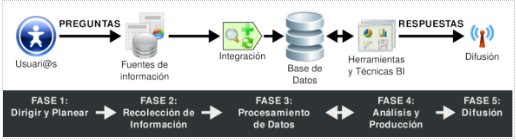
\includegraphics[width=7cm]{imagenes/img1.PNG}

\paragraph{- Fase 1: }

Dirigir y Planear.

En esta fase inicial es donde se deberán recolectar los requerimientos de información específicos de los diferentes 
usuarios, así como entender sus diversas necesidades, para que luego 
en conjunto con ellos se generen las preguntas que les ayudarán a 
alcanzar sus objetivos. 

\paragraph{- Fase 2:}
Recolección de Información.

Es aquí en donde se realiza el proceso de extraer desde las diferentes fuentes de información de la 
empresa, tanto internas como externas, los datos que serán necesarios 
para encontrar las respuestas a las preguntas planteadas en el paso 
anterior. 
\paragraph{- Fase 3:}
Procesamiento de Datos.

En esta fase es donde se integran y 
cargan los datos en crudo en un formato utilizable para el análisis. Esta 
actividad puede realizarse mediante la creación de una nueva base de 
datos, agregando datos a una base de datos ya existente o bien 
consolidando la información. 

\paragraph{- Fase 4:}
Análisis y Producción.

Ahora, se procederá a trabajar sobre 
los datos extraídos integrados, utilizando herramientas y técnicas propias 
de la tecnología BI, para crear inteligencia. Como resultado final de esta 
fase se obtendrán las respuestas a las preguntas, mediante la creación 
de reportes, indicadores de rendimiento, cuadros de mando, gráficos 
estadísticos, etc. 
\paragraph{- Fase 5:}
Difusión.

Finalmente, se les entregará a los usuarios que lo 
requieran las herramientas necesarias, que les permitirán explorar los 
datos de manera sencilla e intuitiva22 

\subsubsection{METODOLOGÍA DE RALPH KIMBALL }
La metodología de Kimball se basa en cuatro principios fundamentales: 
Centrarse en el negocio: Hay que concentrarse en la identificación de 
los requerimientos del negocio y su valor asociado, y usar estos 
esfuerzos para desarrollar relaciones sólidas con el negocio, agudizando 
el análisis del mismo y la competencia consultiva de los 
implementadores. 
Construir una infraestructura de información adecuada: Diseñar una 
base de información única, integrada, fácil de usar, de alto rendimiento 
donde se reflejará la amplia gama de requerimientos de negocio 
identificados en la empresa. 
Realizar entregas en incrementos significativos: crear el almacén de 
datos (DW) en incrementos entregables en plazos de 6 a 12 meses. Hay 
que usa el valor de negocio de cada elemento identificado para 
determinar el orden de aplicación de los incrementos. En esto la 
metodología se parece a las metodologías ágiles de construcción de 
software. 
Ofrecer la solución completa: proporcionar todos los elementos 
necesarios para entregar valor a los usuarios de negocios. Para 
comenzar, esto significa tener un almacén de datos sólido, bien diseñado, 
con calidad probada, y accesible. También se deberá entregar 
herramientas de consulta ad hoc, aplicaciones para informes y análisis 
avanzado, capacitación, soporte, sitio web y documentación. 
La construcción de una solución de DW es compleja, y Kimball propone una 
metodología que ayuda a simplificar dicha solución. Las tareas de esta 
metodología (ciclo de vida) se muestran en la siguiente figura:

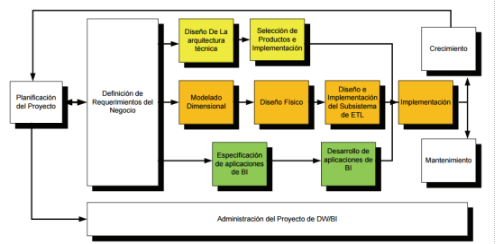
\includegraphics[width=6cm]{imagenes/img2.png}

\subsubsection{METODOLOGÍA CRISP-DM (Cross- Industry Standard PRocess for Data Mining). }
La metodología de CRISP es una de las principales metodologías por seguir por 
los analistas en la inteligencia de negocios, donde se puede rescatar 
primordialmente Data Warehouse y Data Mining. 
La metodología CRISP está sustentada en estándares internacionales que reflejas 
la robustez de sus procesos y que facilitan la unificación de sus fases en una 
estructura confiable y amigable para el usuario. Además de ello, esta tecnología 
interrelaciona las diferentes fases del proceso entre sí, de tal manera que se 
consolida un proceso iterativo y recíproco. Otro aspecto fundamental de esta 
tecnología es que es planteada como una metodología imparcial o “neutra 
respecto a la herramienta que se utilice para el desarrollo del proyecto de Data 
Warehouse o Data Mining siendo su distribución libre y gratuita. 
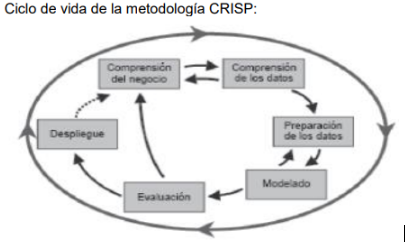
\includegraphics[width=7cm]{imagenes/img3.png}
El ciclo de vida del proyecto según la metodología según la metodología 
de CRISP está basado en seis fases cambiantes entre sí y nunca 
terminantes, lo cual lo postula como un ciclo en constante movimiento. 

\paragraph{- Comprensión del negocio:}
Se trata de entender claramente los 
requerimientos y objetivos del proyecto siempre desde una visión de 
negocio. Esta fase se subdivide a su vez en las siguientes categorías: 
o Definición de los objetivos del negocio (inicial, objetivos de 
negocio y criterios de éxito del negocio). 
o Evaluación de la situación (inventario de recursos, requisitos 
supuestos y requerimientos, riesgos y contingencias, terminología 
y costes y beneficios). 
o Definición de los objetivos del DW (objetivos y criterios de éxito). 
o Realización del plan del proyecto (plan del proyecto y valoración 
inicial de herramientas y técnicas). 

\paragraph{- Comprensión de los datos:}
Es conseguir y habituarse con los datos, 
reconocer las dificultades en la calidad de los datos y reconocer también 
las fortalezas de estos mismos que pueden servir en el proceso de 
análisis. Sus subdivisiones son: 

\begin{itemize}
    \item Recolección inicial de datos (informe de recolección). 
    \item Descubrimiento de los datos (informe descriptivo de los datos).
    \item Exploración de los datos (informe de exploración de los datos).
    \item Verificación de la calidad de los datos (informes de calidad). 
    
\end{itemize}
\subsection{DATA LAKE}
\subsubsection{Concepto}
El Data Lake es un repositorio compartido que le permite adquirir y almacenar grandes cantidades de datos procedentes de sistemas heterogéneos en formato nativo, es decir, datos en bruto estructurados, semiestructurados y no estructurados. La adquisición puede provenir de sistemas heredados, como CRM y ERP, o de fuentes externas, como feeds, Internet de las Cosas y datos de redes sociales.
El propósito de un Data Lake es, por lo tanto, proporcionar una visión no necesariamente refinada de los datos para apoyar las actividades de Data Discovery, lo que lo convierte en un sistema adecuado para usuarios expertos.

\subsubsection{Atributos clave de un data lake}
\begin{itemize}
    \item  Cómputo y almacenamiento desacoplado.
    \item  Ingesta y transformación rápida.
    \item   Seguridad en ambientes multitenant
    \item   Query in place
    \item  Schema on read
\end{itemize}
Los data lakes extienden el enfoque tradicional al tener diversos motores de análisis, almacenamiento a bajo costo, escalas de TBs -EBs

\subsubsection{Capas comunes de data lake(tecnologías)}
\begin{itemize}
    \item  Data Ingestion: capa temporal de carga en la que los datos pasan checks básicos antes de ser almacenados en la capa de raw data. Si bien no es necesaria, se puede implementar para llevar a cabo
    \item  controles básicos de calidad, como posibles filtros según el origen de los datos, descartando fuentes desconocidas
    \item  procesos de encriptación de los datos en caso de requerirse por motivos de seguridad
    \item  registros sencillos de metadata y trazabilidad mediante tags, almacenando el origen de los datos, fecha y hora de carga, el formato y otras características técnicas, su privacidad y nivel de seguridad, algoritmo de encriptación, etc.
    \item Data Storage (Raw Data): capa sin esquema establecido donde todos los datos, estructurados o no estructurados, son almacenados sin sufrir adaptaciones. Es una capa en la que se precisa de analistas expertos en data discovery mediante herramientas big data (Hive, Spark, Map Reduce…).
    \item  Data Processing (Zona de Confianza): Una vez que los analistas de datos han realizado data discovery en el raw data, se puede ver la necesidad de procesar y adaptar determinados sets de datos para alojarlos en una capa de uso recurrente. En esta capa pueden tener lugar procesos avanzados de data quality, integridad y otras adaptaciones para disponer de una capa de confianza de exploración de datos a la que tengan acceso otros usuarios.
    \item   Data Access (Zona de Consumo): esta es una capa más avanzada donde, finalmente, los datos se ponen a disposición de analistas de negocio. Estos analistas podrá generar informes y análisis para responder a preguntas de negocio y afianzar la toma de decisiones. 
\end{itemize}
\subsubsection{Arquitectura de Data lake}
\paragraph{Arquitectura de zona}
\begin{itemize}
    \item De estanque: Inmon diseña un lago de datos como un conjunto de estanques de datos [23]. un dato estanque se puede ver como una subdivisión de un lago de datos que trata con datos de un específico escribe. De acuerdo con las especificaciones de Dixon, cada estanque de datos está asociado con un sistema de almacenamiento especializado, algún procesamiento y acondicionamiento de datos específicos (es decir, transformación/preparación de datos) y un servicio de análisis relevante. Más precisamente, Inmon identifica cinco estanques de datos.
    \item  De zona : Arquitecturas de zona Las denominadas arquitecturas de zona asignan datos a una zona según a su grado de refinamiento.
\end{itemize}
\paragraph{Arquitecturas funcionales y de madurez}
Para superar las contradicciones de la categorización estanque/zona, se propone una forma alternativa de agrupar arquitecturas de lagos de datos con respecto al tipo de criterios Se utiliza para definir componentes. Como resultado, distinguimos arquitecturas funcionales, arquitecturas basadas en la madurez de datos y arquitecturas híbridas

\subsubsection{Ventajas de Data lake}
\begin{itemize}
    \item El Data Lake permite centralizar todos los datos en un mismo lugar, vengan de la fuente que vengan. Una vez incluidas en su silo correspondiente de información, pueden ser procesadas a través de herramientas de Big Data. Muchas veces, en esa disparidad de información, habrá datos que requieran un tratamiento especial en cuanto a seguridad. Gracias al Data Lake, este aspecto se puede solventar.
    \item  Puede que la fuente original del dato esté obsoleta o se haya desactivado, sin embargo, su contenido puede que siga siendo valioso para el análisis. A través del Data Lake, puedes acceder a dicha información.
    \item  Todo dato que llegue al Data Lake puede ser normalizado y enriquecido.
    \item  Los datos se preparan en función de la necesidad del momento. Esto permite reducir considerablemente los costes y los tiempos. En el Data Warehouse, por ejemplo, es necesaria dicha preparación.
    \item  Se puede acceder a la información y enriquecerla desde cualquier punto del planeta, por cualquier usuario autorizado por el Data Lake. Esto ayuda a la organización a recopilar más fácilmente los datos necesarios para la toma de decisiones.
    \item  Un Data Lake pone la información en manos de un mayor número de personas dentro de cualquier organización, aprovechándose mejor la empresa de ese conocimiento que adquieren dichos individuos.
\end{itemize}
\subsection{Comparativa Data lake y Data Warehouse}

\begin{itemize}
    \item  Los data lake y los data warehouse se utilizan de forma generalizada para el almacenaje de big data, pero, aunque ambos son almacenes de datos, estos no son términos intercambiables. Un data lake o "lago de datos" es un gran conjunto de datos en bruto, que todavía no tiene una finalidad definida. En cambio, un data warehouse o "almacén de datos" es un depósito de datos que ya están estructurados y filtrados y han sido procesados para un propósito concreto.
    \item   Datalake conserva todos los datos, a diferencia del almacén de datos, donde se dedica una parte importante de tiempo a decidir qué datos incluir y no incluir en el almacén.
    \item Data Lake admite todos los tipos de datos, independientemente de su tipo, formato o procedencia y sin necesidad de normalizar su estructura. La información se mantiene en su forma original y solo se transforma cuando se va a consumir.
    \item   Data Lake puede nutrir a todos los usuarios de la organización, incluyendo a esos perfiles técnicos con exigencias de análisis más avanzadas, que son quienes recurren a capacidades como análisis estadístico y modelado predictivo.
    \item   A diferencia del Data Warehouse, el Data Lake se adapta fácilmente a los cambios. El diseño del almacén es un proceso complejo y, la actualidad de loso negocios, en ocasiones no puede esperar tanto tiempo. Para esas circunstancias, asegura la adaptabilidad necesaria para entregar respuestas más rápidas.
\end{itemize}


\section{Conclusiones}

Es necesario revisar la categorías de un lago de datos y un almacén de datos, para analizar cual adapta mejor al caso de uso en el que se desea trabajar.
Cuando se construyen tuberías de datos, es necesario implementar una combinación de ambas soluciones de almacenamiento.


\section{Recomendaciones}
 El lago de datos integran diferentes tipos de datos para generar preguntas completamente nuevas, ya que es probable que estos usuarios no usen almacenes de datos porque pueden necesitar ir más allá de sus capacidades, mientras que en el almacén de datos la mayoría de los usuarios de una organización están operativos. Este tipo de usuarios solo se preocupa por los informes y las métricas clave de rendimiento.

 
 


%----------------------------------------------------------------------------------------
%	REFERENCE LIST
%----------------------------------------------------------------------------------------
\begin{thebibliography}{}

    \bibitem{DOC2008} 
    Data Lake vs Data Warehouse. Veamos sus principales diferencias. (2022). Powerdata.es. https://blog.powerdata.es/el-valor-de-la-gestion-de-datos/data-lake-vs-data-warehouse.-veamos-sus-principales-diferencias
    \bibitem{FRE2016} 
   Gorini, M. (2022). ¿Cuál es la diferencia entre un data lake y un data warehouse? Bismart.com. http://blog.bismart.com/diferencia-entre-data-lake-y-data-warehouse
	\bibitem{FRE2016} 
   Gigliotti, M. (2019). Data Lake y Data Warehouse: ¿Qué son y en qué se diferencian? Techedgegroup.com. https://www.techedgegroup.com/es/blog/data-lake-data-warehouse-definicion-diferencias
    \bibitem{FRE2019} 
   Data Lake vs Data Warehouse: Key Differences - Talend. (2022). Talend - a Leader in Data Integration Data Integrity. https://www.talend.com/resources/data-lake-vs-data-warehouse/
  
    \bibitem{FRE2019}
    Emilio Fernández Lastra. (2018, October 10). Data Warehouse y Data Lake. Qué son y para qué sirven. Artyco | the Data Driven Company. https://artyco.com/data-warehouse-data-lake-que-es/
    
    \bibitem{FRE2018}
   Prakash, S. S. (2020, April). Evolution of Data Warehouses to Data Lakes for Enterprise Business Intelligence. ResearchGate; unknown. https://www.researchgate.net/publication/343219651EvolutionofDataWarehousestoDataLakesforEnterpriseBusinessIntelligence/link/5f1d52ad92851cd5fa48958a/download
   
   \bibitem{FRE2018}
  Flores, A. (n.d.). Construyendo y governando Data Lakes y Data Warehouses modernos en AWS. Retrieved April 5, 2022, from https://d1.awsstatic.com/events/Summits/AMER2019/Mexico-City/BuildingandgoverningmoderndatalakesanddatawarehousesADB201.pdf
   
   \bibitem{FRE2018}
   Mendez, A., Britos, A.,  Garcia-Martínez, P. Y. (2003). Fundamentos de Data Warehouse. Reportes Técnicos En Ingeniería Del Software, 5(1), 19–26. http://artemisa.unicauca.edu.co/~ecaldon/docs/bd/fundamentosdedatawarehouse.pdf
    
    \bibitem{FRE2018}
    Agudelo, J. (2020) Data Lakes: Aplicaciones, Herramientas y Arquitecturas. Monografía presentada como requisito para optar al Título de Ingeniero de Sistemas y Computación https://repositorio.utp.edu.co/server/api/core/bitstreams/5f56e572-d416-487e-a6d5-ec3a8e45da46/content
 
	\bibitem{FRE2018}
	Pegdwendé Sawadogo, Jérôme Darmont. On data lake architectures and metadata management. Journal of Intelligent Information Systems, Springer Verlag, 2021, 56 (1), pp.97-120. ff10.1007/s10844- 020-00608-7ff. ffhal-03114365f https://hal.archives-ouvertes.fr/hal-03114365/document


 
    \end{thebibliography}


%----------------------------------------------------------------------------------------

\end{document}